\clearpage
\section{M-QAM Transmission System}

\begin{tcolorbox}	
	\begin{tabular}{p{2.75cm} p{0.2cm} p{10.5cm}} 	
		\textbf{Student Name}  &:& Ana Luisa Carvalho\\
		\textbf{Goal}          &:& M-QAM system implementation with BER measurement and comparison with theoritical values.\\
		\textbf{Directory} &:& sdf/m\_qam\_system
	\end{tabular}
\end{tcolorbox}

M-QAM, which stands for Quadrature Amplitude Modulation, is a modulation scheme that takes advantage of two carriers (usually sinusoidal waves) with a phase difference of $\frac{\pi}{2}$. The resultant output consists of a signal with both amplitude and phase variations. The two carriers, refered to as I (In-phase) and Q (Quadrature), can be represented as 

\begin{align}
	I=A\cos(\phi) \\
	Q=A\sin(\phi)
\end{align}
which means that any sinusoidal wave can be decomposed in its I and Q components:

\begin{align}
A\cos(\omega~t+\phi)&=A\left(\cos(\omega~t)\cos(\phi)-\sin(\omega~t)\sin(\phi)\right) \\
&=I\cos(\omega~t)-Q\sin(\omega~t),
\end{align} 
where we have used the expression for the cossine of a sum and the definitions of I and Q.

For M$=4$ the symbol constellation is shown figure \ref{fig:const}.

The goal of this project is to simulate a M-QAM transmission system and to perform a Bit Error Rate (BER) measurement that can be compared with theoretical values. 

\begin{figure}[h]
	\centering
	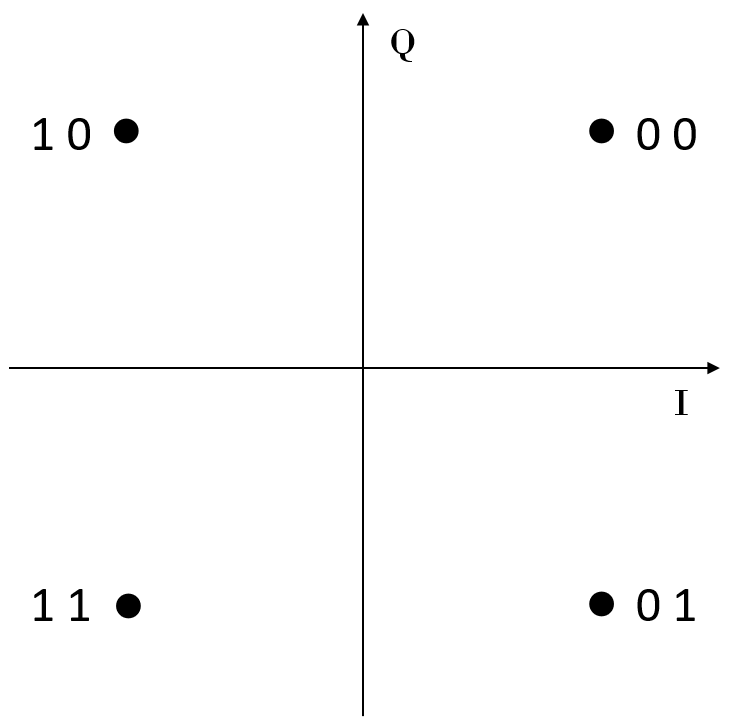
\includegraphics[width=0.5\textwidth]{./figures/MQAM_constellation}
	\caption{4-QAM symbol constellation}
	\label{fig:const}
\end{figure}

%M can take several values: $2, 4, 16, 32, ...$. The first two correspond to BPSK and QPSK modulation, respectively.

\subsection{Theoretical Analysis }

%When demodulating a signal it is necessary to associate the received signal to the corresponding signal. The existence of noise in the channel means that we can only compute the probability that a given signal corresponds to a certain carrier and that's why we need to define the BER. Using
%
%\begin{equation}
%P_i f(s|c_i)>P_j f(s|c_j), \qquad i\neq j
%\end{equation}
%where $f(s|c_i)$ stands for the probability of detecting the signal $s$ given that $c_i$ was emmited. This inequallity can be rewritten in the following way
%
%\begin{equation}
%P(c_i|s)>P(c_j|s)
%\end{equation}
%where $P(c_i|s)$ and $P(c_j|s)$ are called \textit{a posteriori} probabilities and represent the probability that $c_i$ or $c_j$ were transmitted given that $s$ was received. In terms of the systems this simply means that we should select the signal most likely to have been transmitted.
%
%In the case of additive white gaussian noise the $f$ function is simply given by
%
%\begin{equation}
%f(s|c_i)=\frac{e^{-x^2/n_0}}{(\pi n_0)^{N/2}}
%\end{equation}
%where $x$ is the Euclidean distance in the I-Q plane between the signal received and carrier i and $N$ is the number of noise samples.
%
%When using 4-QAM modulation all points are at an equal distance from the origin (in the I-Q plane) so they all have the same energy given by
%
%\begin{equation}
%E=\frac{d^2}{2}
%\end{equation}
%where $d$ is the side of the square formed bye the constellation points.
%
%The probability that a given signal is identified correctly is given by
%
%\begin{equation}
%P_c=r^2
%\end{equation}
%where $n_0/2$ is the noise variance for AWGN and
%
%\begin{equation}
%r=\int_{-d/2}^{\infty}\frac{e^{-x^2/n_0}}{\sqrt{\pi n_0}} dx.
%\end{equation}
%
%The error probability, $P_e$, given by $1-P_c$ is given by
%
%\begin{equation}
%P_e=\erfc \sqrt{\frac{E}{2 n_0}}.
%\end{equation}

The probability of symbol error, $P_s$, in coherent M-PSK demodulation with additive white gaussian nois is given by 

\begin{equation}
	P_s=2~Q\left(\sqrt{2~\log_2 M \left(\frac{E_b}{n_0}\right)\sin^2\frac{\pi}{M}}\right)
\end{equation}
where $E_b$ is the energy of one bit, $n_0$ is the noise power and the function $Q$ is defined as
\begin{equation}
	Q(x)=\frac{1}{2} erfc\left(\frac{x}{\sqrt{2}}\right).
	\label{eq:Ps}
\end{equation}

The probability of bit errors, $P_b$ is related to $P_s$ by
\begin{equation}
	P_b=\frac{1}{\log_2 M}P_s.
	\label{eq:Pb}
\end{equation} 

For QPSK we get, using $M=4$ in equations \ref{eq:Ps} and \ref{eq:Pb},
\begin{equation}
	P_b=\frac{1}{2} erfc\left(\sqrt{\frac{2~E_b}{n_0}}\right).
\end{equation}

This function is plotted in figure \ref{fig:QPSK_th_curve} for $n_0=10^6$.

\begin{figure}
		\centering
		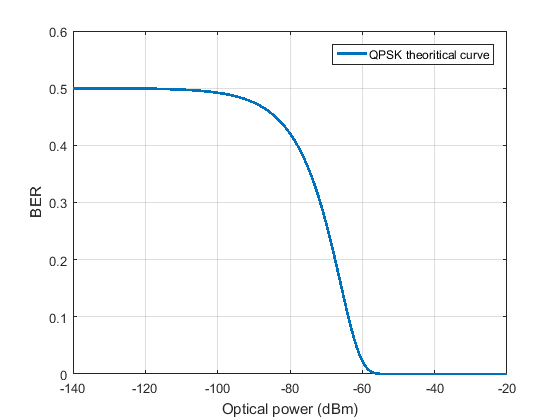
\includegraphics[width=0.8\textwidth]{./figures/QPSK_th_curve}
		\caption{QPSK theoretical BER}
		\label{fig:QPSK_th_curve}
\end{figure}
\subsection{Simulation Analysis}

The M-QAM transmission system is a complex block of code that simulates the modulation, transmission and
demodulation of an optical signal using M-QAM modulation.
It is composed of four blocks: a transmitter, a receiver, a sink and a block that performs a Bit Error Rate (BER) measurement. The schematic representation of the
system is presented in figure \ref{MQAM_system_block_diagram}. 

\begin{figure}
	\centering
	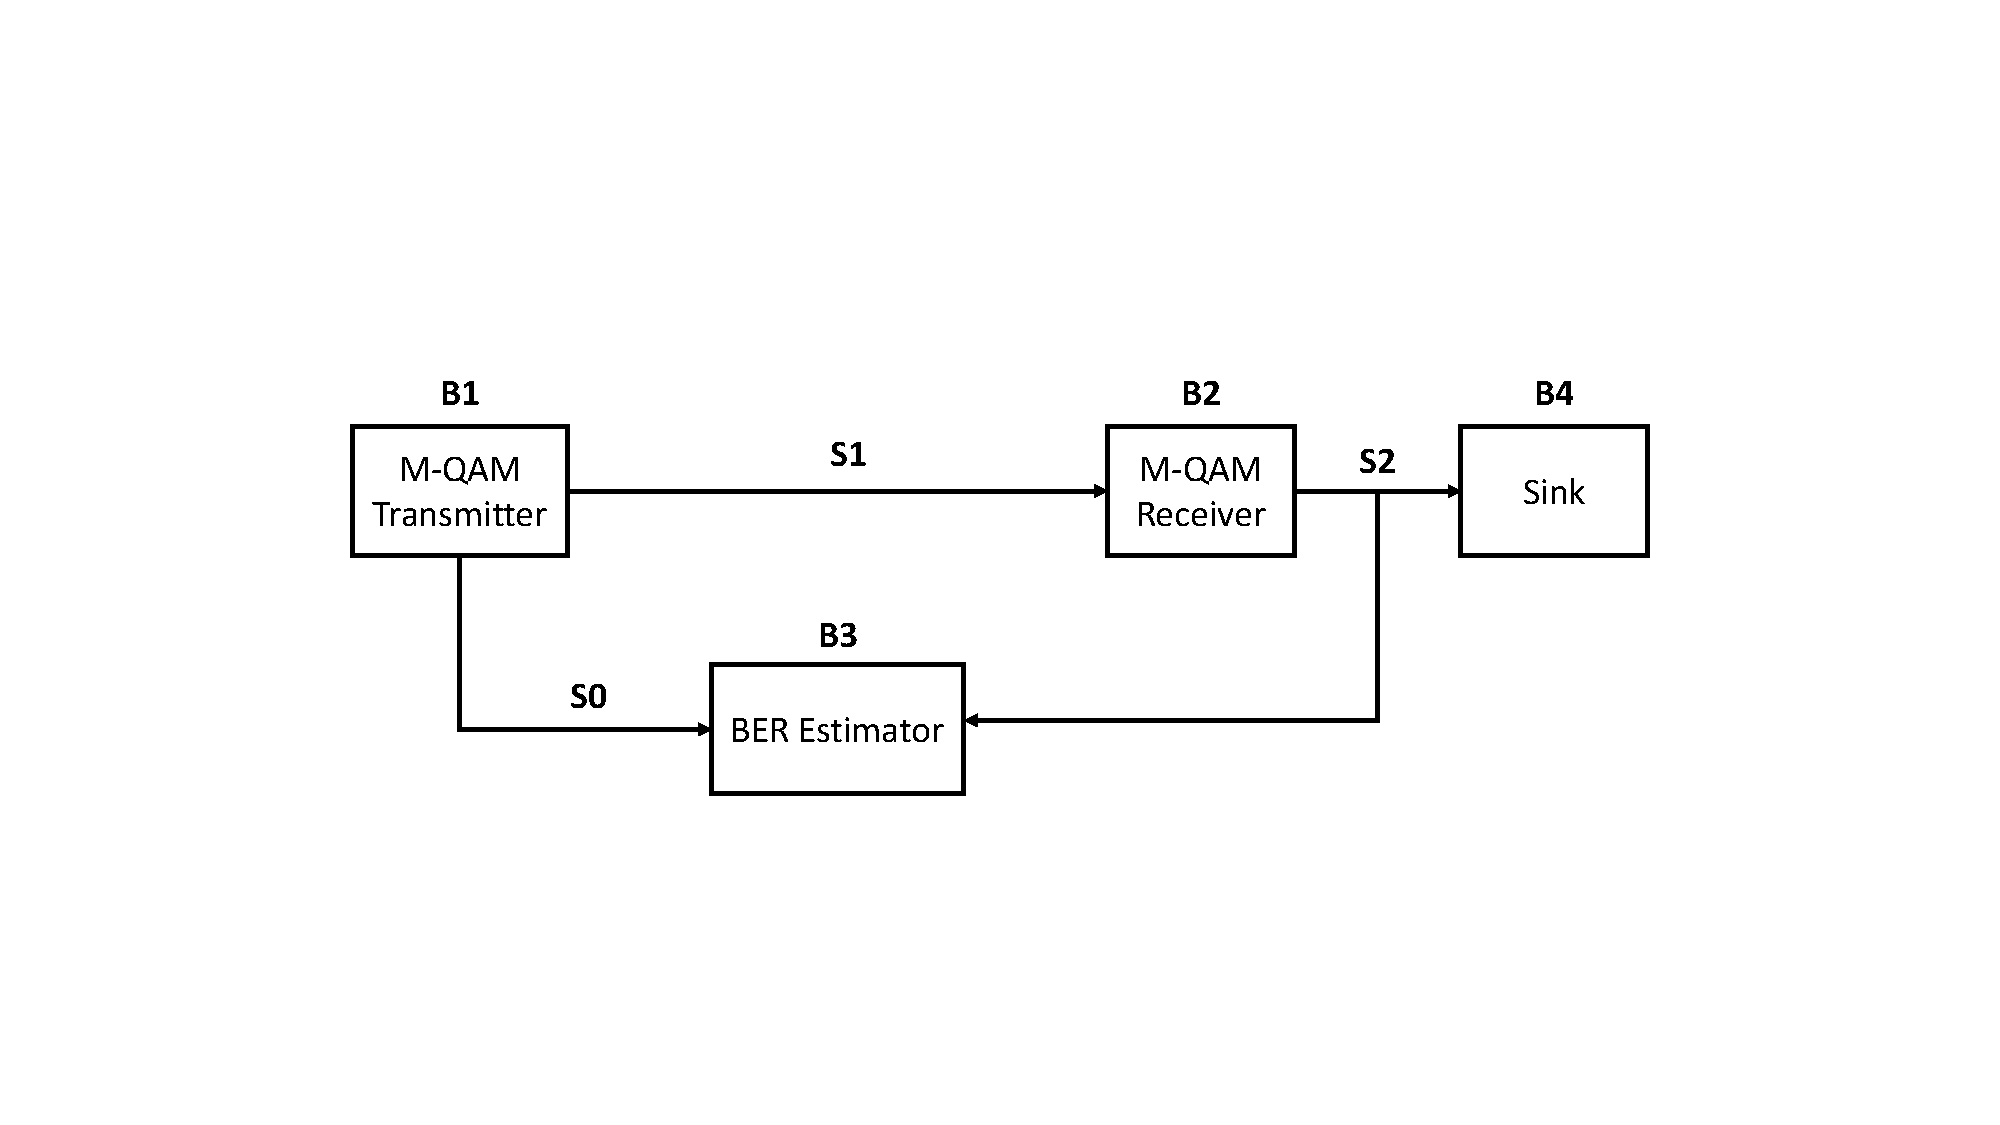
\includegraphics[width=0.8\textwidth]{./figures/MQAM_system_block_diagram}
	\caption{Schematic representation of the MQAM system.}\label{MQAM_system_block_diagram}
\end{figure}

\paragraph{Current state:} The system currently being implement is a QPSK system (M=4).

\paragraph{Future work:} Extend this block to include other values of M.

\subsection*{Functional description}

A complete description of the M-QAM transmitter and M-QAM homodyne receiver blocks can be found in the \textit{Library} chapter of this document as well as a detailed description of the independent blocks that compose these blocks.

The M-QAM transmitter generates one or two optical signals by enconding a binary string using M-QAM modulation. It also outputs a binary signal that is used to perform the BER measurement.

The M-QAM homodyne receiver accepts one input optical signal and outputs
a binary signal. It performs the M-QAM demodulation of the input signal by combining the optical signal with a local oscillator.

The demodulated optical signal is compared to the one produced by the transmitter in order to estimate the Bit Error Rate (BER).

The files corresponding to each of the system's blocks are summarized in table \ref{files_table}. Along with the library and corresponding source files these allow for the full operation of the M-QAM system described here.

\begin{table}[]
	\centering
	\label{files_table}
	\caption{Main system files}
	\begin{tabular}{|c|c|c|ccc}
		\cline{1-3}
		\textbf{System blocks} & \textbf{Source file} & \textbf{Header file}  &  \\ \cline{1-3}
		Main & m\_qam\_system\_sdf.cpp & --- &  \\ \cline{1-3}
		M-QAM transmitter & m\_qam\_transmitter.cpp & m\_qam\_transmitter.h &  \\ \cline{1-3}
		M-QAM receiver & homodyne\_receiver.cpp & homodyne\_receiver.h &   \\ \cline{1-3}
		Sink & sink.cpp & sink.h &   \\ \cline{1-3}
		BER estimator & bit\_error\_rate.cpp & bit\_error\_rate.h &  \\ \cline{1-3}
	\end{tabular}
\end{table}

\subsection*{Required Files}

The required header and source files needed to run this system are summarized in table \ref{table:files}.

\begin{table}[]
 	\centering
 	\caption{Required files}
 	\begin{tabular}{|c|c|p{50mm}|ccp{50mm}}
 		\cline{1-3}
 		\textbf{Header file} & \textbf{Source file} & \textbf{Description} &    \\ \cline{1-3}
 		add.h & add.cpp & Add two signals  &    \\ \cline{1-3}
 		binary\_source.h & binary\_source.cpp & Produces a binary sequence \\ \cline{1-3}
 		bit\_error\_rate.h & bit\_error\_rate.cpp & Computes the BER and writes it to a text file \\ \cline{1-3}
 		discrete\_to\_continuous\_time.h & discrete\_to\_continuous\_time.cpp & Takes a signal discrete in time and produces a signal continuous in time \\ \cline{1-3}
 		homodyne\_receiver.h & m\_qam\_homodyne\_receiver.cpp & \\ \cline{1-3}
 		ideal\_amplifier.h & ideal\_amplifier.cpp & Amplifies the signal \\ \cline{1-3}
 		iq\_modulator.h & iq\_modulator.cpp & Divides the signal in its quadrature and in phase components \\ \cline{1-3}
 		local\_oscillator.h & local\_oscillator.cpp & & \\ \cline{1-3}
 		m\_qam\_mapper.h & m\_qam\_mapper.cpp & Maps the signal using the defined constellation \\ \cline{1-3}
 		m\_qam\_transmitter.h & m\_qam\_transmitter.cpp & & \\ \cline{1-3}
 		netxpto.h & netxpto.cpp & General class \\ \cline{1-3}
 		optical\_hybrid.h & optical\_hybrid.cpp & Implements an optical hybrid \\ \cline{1-3}
 		photodiode\_old.h & photodiode\_old.cpp & pair of photodiodes and current subtraction \\ \cline{1-3}
 		pulse\_shaper.h & pulse\_shaper.cpp & Electrical filter \\ \cline{1-3}
 		sampler\_20171119.h & sampler\_20171119.cpp & Samples the signal \\ \cline{1-3}
 		sink.h & sink.cpp & Deletes signal \\ \cline{1-3}
 		super\_block\_interface.h & super\_block\_interface.cpp & & \\ \cline{1-3}
 		white\_noise.h & white\_noise.cpp & Generates white gaussian noise \\ \cline{1-3}  
 	\end{tabular}
 	\label{table:files}
\end{table}

\subsection*{Input Parameters}

The system can take several input parameters. These are described in table \ref{table:in_par}.

\begin{table}[]
	\centering
	\caption{Input parameters}
	\begin{tabular}{|c|c|p{60mm}|ccp{60mm}}
		\cline{1-3}
		\textbf{Parameter} & \textbf{Type} & \textbf{Description} &    \\ \cline{1-3}
		numberOfBitsGenerated & t\_integer & Determines the number of bits to be generated by the binary source  &    \\ \cline{1-3}
		samplesPerSymbol & t\_integer & Number of samples per symbol &    \\ \cline{1-3}
		prbsPatternLength & int & Determines the length of the pseudorandom sequence pattern (used only when the binary source is operated in \textit{PseudoRandom} mode) &    \\ \cline{1-3}
		bitPeriod & t\_real & Temporal interval occupied by one bit &    \\ \cline{1-3}
		rollOffFactor & t\_real & Parameter of the raised cosine filter &    \\ \cline{1-3}
		signalOutputPower\_dBm & t\_real & Determines the power of the output optical signal in dBm &  \\ \cline{1-3}
		numberOfBitsReceived & int &   Determines when the simulation should stop. If $-1$ then it only stops when there is no more bits to be sent&   \\ \cline{1-3}
		iqAmplitudeValues & vector<t\_iqValues> & Determines the constellation used to encode the signal in IQ space &    \\ \cline{1-3}
		symbolPeriod & double & Given by bitPeriod/samplesPerSymbol &    \\ \cline{1-3}
		localOscillatorPower\_dBm & t\_real & Power of the local oscillator &    \\ \cline{1-3}
		responsivity & t\_real & Responsivity of the photodiodes (1 corresponds to having all optical power transformed into electrical current) &    \\ \cline{1-3}
		amplification & t\_real & Amplification provided by the ideal amplifier &    \\ \cline{1-3}
		noiseAmplitude & t\_real & Amplitude of the white noise &    \\ \cline{1-3}
		samplesToSkip & t\_integer & Number of samples to be skipped by the \textit{sampler} block &    \\ \cline{1-3}
		confidence & t\_real & Determines the confidence limits for the BER estimation &    \\ \cline{1-3}
		midReportSize & t\_integer &  &    \\ \cline{1-3}
		bufferLength & t\_integer & Corresponds to the number of samples that can be processed in each run of the system &    \\ \cline{1-3}
		\end{tabular}
		\label{table:in_par}
		\end{table}

\subsection*{Block Output}

As output the system produces text files with all the signals (inputs and outputs of each block). These can be visualized using the visualization tool described in this document. It also produces a text file with the BER estimation. 

\subsection*{Simulation results}

\subsection{Comparative Analysis}

In this section we show the simulation results and compared them with the theoretical predictions. Figures \ref{fig:ber_random} and \ref{fig:ber_det} show the variation of the BER with the power of the signal, using $4000$ bits and a random and deterministic cyclic ($0101...$) binary sequence, respectively. To produce this plots we considered a noise amplitude of $10^{-6}$ and an amplification of $10^3$. 

	\begin{figure}[h]
		\centering
		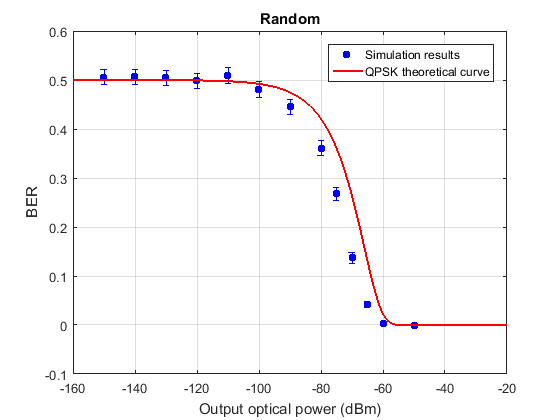
\includegraphics[width=0.8\textwidth]{./figures/QPSK_BER_random}
		\caption{Simulation result for a random binary sequence with $4000$ bits, a noise amplitude of $10^{-6}$ and an amplification of $10^3$}
		\label{fig:ber_random}
	\end{figure}%
	\begin{figure}[h]
		\centering
		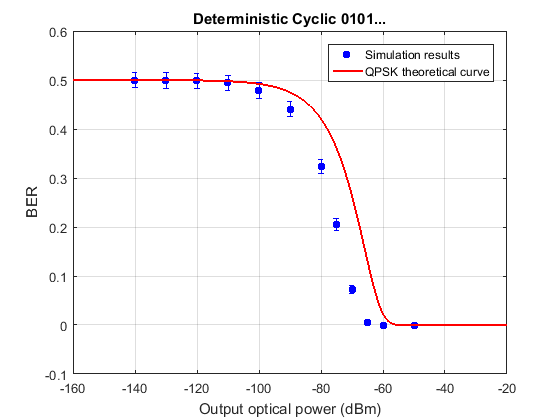
\includegraphics[width=0.8\textwidth]{./figures/QPSK_BER_deterministic_cyclic}
		\caption{Simulation results for a deterministic cyclic binary sequence (0101...) with $4000$ bits, a noise amplitude of $10^{-6}$ and an amplification of $10^3$}
		\label{fig:ber_det}
	\end{figure}




